\section{Supplementary}
\begin{table*}[t]
  \caption{Spearman correlation table for first four samples and their subsamples.}
  \label{speartable}
  \tabcolsep=0pt%%
  \begin{tabular*}{\textwidth}{@{\extracolsep{\fill}}lrrrrrrrr@{\extracolsep{\fill}}}
  \toprule%
  \textbf{} &
  \multicolumn{1}{l}{Sample $1_{01}$} &
  \multicolumn{1}{l}{Sample $1_{02}$} &
  \multicolumn{1}{l}{Sample $2_{01}$} &
  \multicolumn{1}{l}{Sample $2_{02}$} &
  \multicolumn{1}{l}{Sample $3_{01}$} &
  \multicolumn{1}{l}{Sample $3_{02}$} &
  \multicolumn{1}{l}{Sample $4_{01}$} &
  \multicolumn{1}{l}{Sample $4_{02}$} \\
EM           & 0.932 & 0.932 & 0.933 & 0.932 & 0.937 & 0.936 & 0.934 & 0.933 \\
both - $10^{-5}$ & 0.933 & 0.933 & 0.934 & 0.933 & 0.939 & 0.938 & 0.935 & 0.934 \\
VBEM - $10^{-5}$ & 0.952 & 0.951 & 0.953 & 0.951 & 0.957 & 0.956 & 0.954 & 0.952 \\
both - $10^{-4}$ & 0.933 & 0.933 & 0.934 & 0.933 & 0.939 & 0.938 & 0.935 & 0.934 \\
VBEM - $10^{-4}$ & 0.952 & 0.951 & 0.953 & 0.951 & 0.957 & 0.956 & 0.954 & 0.952 \\
both - $10^{-3}$ & 0.933 & 0.933 & 0.934 & 0.933 & 0.939 & 0.938 & 0.935 & 0.934 \\
VBEM - $10^{-3}$ & 0.952 & 0.951 & 0.953 & 0.951 & 0.957 & 0.956 & 0.954 & 0.952 \\
both - $10^{-2}$ & 0.933 & 0.933 & 0.934 & 0.933 & 0.939 & 0.938 & 0.935 & 0.934 \\
VBEM - $10^{-2}$ & 0.952 & 0.951 & 0.953 & 0.952 & 0.957 & 0.956 & 0.954 & 0.952 \\
both - $10^{-1}$ & 0.933 & 0.933 & 0.934 & 0.933 & 0.939 & 0.937 & 0.935 & 0.934 \\
VBEM - $10^{-1}$ & 0.951 & 0.950 & 0.953 & 0.951 & 0.957 & 0.955 & 0.954 & 0.951 \\
both - $10^{0}$  & 0.755 & 0.754 & 0.755 & 0.754 & 0.755 & 0.755 & 0.755 & 0.754 \\
VBEM - $10^{0}$  & 0.751 & 0.751 & 0.751 & 0.751 & 0.752 & 0.752 & 0.751 & 0.751 \\
both - $10^{1}$  & 0.736 & 0.735 & 0.736 & 0.736 & 0.738 & 0.737 & 0.736 & 0.736 \\
VBEM - $10^{1}$  & 0.715 & 0.715 & 0.715 & 0.716 & 0.717 & 0.717 & 0.715 & 0.715 \\
  \botrule
  \end{tabular*}
  % \begin{tablenotes}%
  % \item Note: This is an example of table footnote this is an example of table footnote this is an example of table footnote this is an example of~table footnote this is an example of table footnote
  % \item[$^{1}$] Example for a first table footnote.
  % \item[$^{2}$] Example for a second table footnote.\vspace*{6pt}
  % \end{tablenotes}
  \end{table*}

  

  \begin{table*}[t]
    \caption{MARD table for first four samples and their subsamples.}
    \label{mardtable}
    \tabcolsep=0pt%%
    \begin{tabular*}{\textwidth}{@{\extracolsep{\fill}}lrrrrrrrr@{\extracolsep{\fill}}}
    \toprule%
    \textbf{} &
    \multicolumn{1}{l}{Sample $1_{01}$} &
    \multicolumn{1}{l}{Sample $1_{02}$} &
    \multicolumn{1}{l}{Sample $2_{01}$} &
    \multicolumn{1}{l}{Sample $2_{02}$} &
    \multicolumn{1}{l}{Sample $3_{01}$} &
    \multicolumn{1}{l}{Sample $3_{02}$} &
    \multicolumn{1}{l}{Sample $4_{01}$} &
    \multicolumn{1}{l}{Sample $4_{02}$} \\
  EM           & 0.284 & 0.285 & 0.273 & 0.276 & 0.243 & 0.245 & 0.277 & 0.278 \\
  both - $10^{-5}$ & 0.287 & 0.287 & 0.275 & 0.278 & 0.245 & 0.247 & 0.279 & 0.280 \\
  VBEM - $10^{-5}$ & 0.241 & 0.243 & 0.229 & 0.232 & 0.199 & 0.201 & 0.233 & 0.235 \\
  both - $10^{-4}$ & 0.287 & 0.287 & 0.275 & 0.278 & 0.245 & 0.247 & 0.279 & 0.280 \\
  VBEM - $10^{-4}$ & 0.241 & 0.243 & 0.229 & 0.232 & 0.199 & 0.201 & 0.233 & 0.235 \\
  both - $10^{-3}$ & 0.287 & 0.287 & 0.275 & 0.278 & 0.245 & 0.247 & 0.279 & 0.280 \\
  VBEM - $10^{-3}$ & 0.241 & 0.243 & 0.229 & 0.232 & 0.199 & 0.201 & 0.232 & 0.235 \\
  both - $10^{-2}$ & 0.287 & 0.287 & 0.275 & 0.278 & 0.244 & 0.247 & 0.279 & 0.280 \\
  VBEM - $10^{-2}$ & 0.241 & 0.243 & 0.229 & 0.232 & 0.198 & 0.201 & 0.232 & 0.235 \\
  both - $10^{-1}$ & 0.286 & 0.287 & 0.274 & 0.277 & 0.244 & 0.246 & 0.278 & 0.280 \\
  VBEM - $10^{-1}$ & 0.241 & 0.243 & 0.229 & 0.232 & 0.199 & 0.201 & 0.233 & 0.235 \\
  both - $10^0$  & 0.663 & 0.662 & 0.658 & 0.658 & 0.647 & 0.647 & 0.660 & 0.660 \\
  VBEM - $10^0$  & 0.662 & 0.662 & 0.658 & 0.658 & 0.647 & 0.647 & 0.660 & 0.659 \\
  both - $10^1$  & 0.663 & 0.663 & 0.660 & 0.659 & 0.651 & 0.650 & 0.662 & 0.660 \\
  VBEM - $10^1$  & 0.678 & 0.678 & 0.675 & 0.674 & 0.667 & 0.666 & 0.677 & 0.675

    \botrule
    \end{tabular*}
    % \begin{tablenotes}%
    % \item Note: This is an example of table footnote this is an example of table footnote this is an example of table footnote this is an example of~table footnote this is an example of table footnote
    % \item[$^{1}$] Example for a first table footnote.
    % \item[$^{2}$] Example for a second table footnote.\vspace*{6pt}
    % \end{tablenotes}
    \end{table*}
  
    

% \begin{figure*}[!t]%
%     \centering
%     {        
%         \begin{table}[]
%             \begin{tabular}{lrrrrrrrr}
%             \textbf{} &
%               \multicolumn{1}{l}{Sample $1_{01}$} &
%               \multicolumn{1}{l}{Sample $1_{02}$} &
%               \multicolumn{1}{l}{Sample $2_{01}$} &
%               \multicolumn{1}{l}{Sample $2_{02}$} &
%               \multicolumn{1}{l}{Sample $3_{01}$} &
%               \multicolumn{1}{l}{Sample $3_{02}$} &
%               \multicolumn{1}{l}{Sample $4_{01}$} &
%               \multicolumn{1}{l}{Sample $4_{02}$} \\
%             EM           & 0.284 & 0.285 & 0.273 & 0.276 & 0.243 & 0.245 & 0.277 & 0.278 \\
%             both - $10^{-5}$ & 0.287 & 0.287 & 0.275 & 0.278 & 0.245 & 0.247 & 0.279 & 0.280 \\
%             VBEM - $10^{-5}$ & 0.241 & 0.243 & 0.229 & 0.232 & 0.199 & 0.201 & 0.233 & 0.235 \\
%             both - $10^{-4}$ & 0.287 & 0.287 & 0.275 & 0.278 & 0.245 & 0.247 & 0.279 & 0.280 \\
%             VBEM - $10^{-4}$ & 0.241 & 0.243 & 0.229 & 0.232 & 0.199 & 0.201 & 0.233 & 0.235 \\
%             both - $10^{-3}$ & 0.287 & 0.287 & 0.275 & 0.278 & 0.245 & 0.247 & 0.279 & 0.280 \\
%             VBEM - $10^{-3}$ & 0.241 & 0.243 & 0.229 & 0.232 & 0.199 & 0.201 & 0.232 & 0.235 \\
%             both - $10^{-2}$ & 0.287 & 0.287 & 0.275 & 0.278 & 0.244 & 0.247 & 0.279 & 0.280 \\
%             VBEM - $10^{-2}$ & 0.241 & 0.243 & 0.229 & 0.232 & 0.198 & 0.201 & 0.232 & 0.235 \\
%             both - $10^{-1}$ & 0.286 & 0.287 & 0.274 & 0.277 & 0.244 & 0.246 & 0.278 & 0.280 \\
%             VBEM - $10^{-1}$ & 0.241 & 0.243 & 0.229 & 0.232 & 0.199 & 0.201 & 0.233 & 0.235 \\
%             both - $10^0$  & 0.663 & 0.662 & 0.658 & 0.658 & 0.647 & 0.647 & 0.660 & 0.660 \\
%             VBEM - $10^0$  & 0.662 & 0.662 & 0.658 & 0.658 & 0.647 & 0.647 & 0.660 & 0.659 \\
%             both - $10^1$  & 0.663 & 0.663 & 0.660 & 0.659 & 0.651 & 0.650 & 0.662 & 0.660 \\
%             VBEM - $10^1$  & 0.678 & 0.678 & 0.675 & 0.674 & 0.667 & 0.666 & 0.677 & 0.675
%             \end{tabular}
%             \end{table}

%     }
%     \caption{MARD table for first four samples and their subsamples.}
%     \label{mardtable}
% \end{figure*}


% \includesvg{"Min, Median, and Max MARD.svg"}
% \includesvg{"Min, Median, and Max Spearman Correlation.svg"}

\begin{figure*}[!t]%
\centering
{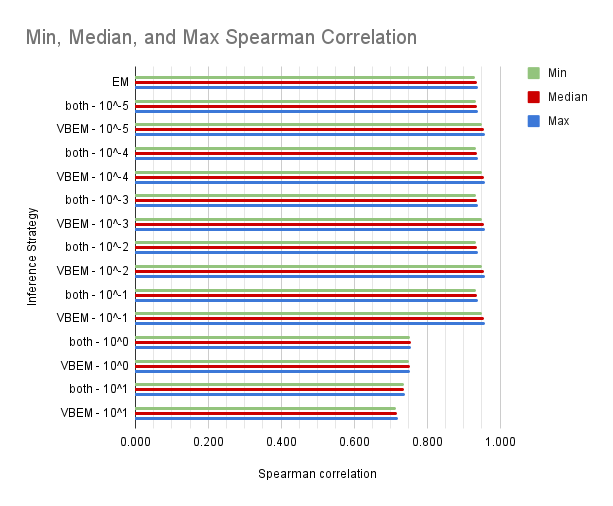
\includegraphics[width=\textwidth]{Min, Median, and Max Spearman Correlation.png}}
\caption{Min, Median, and Max Spearman Correlation}\label{spearfig}
\end{figure*}

\begin{figure*}[!t]%
  \centering
  {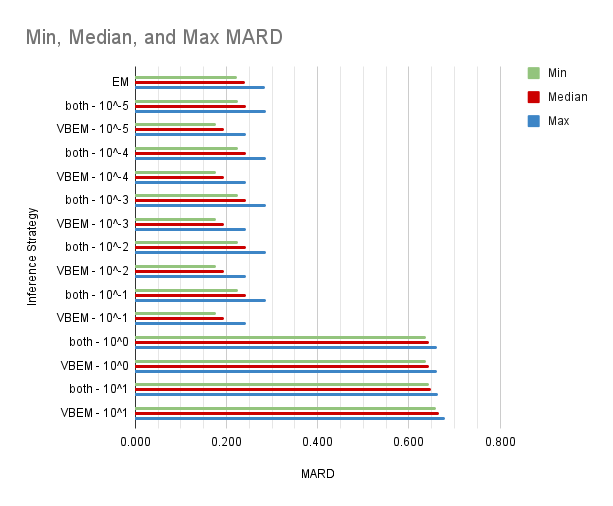
\includegraphics[width=\textwidth]{Min, Median, and Max MARD.png}}
  \caption{Min, Median, and Max MARD}\label{mardfig}
  \end{figure*}
% \begin{figure}
%     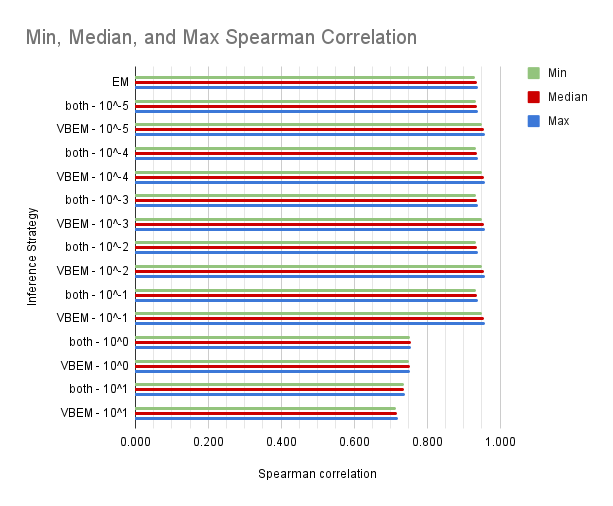
\includegraphics{Min, Median, and Max Spearman Correlation.png}
% \end{figure}
% \begin{figure}
% 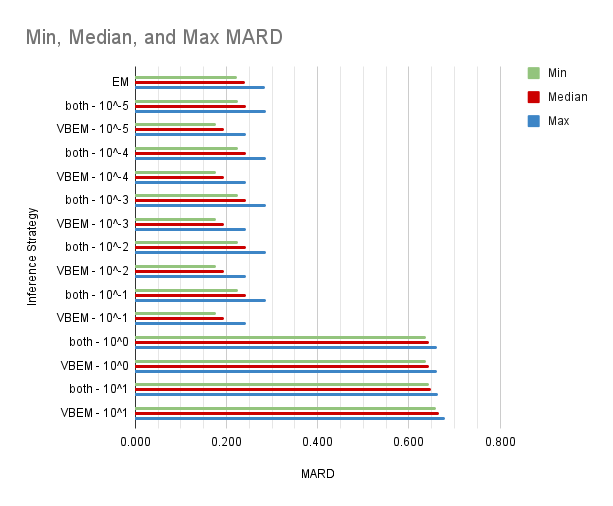
\includegraphics{Min, Median, and Max MARD.png}
% \end{figure}